\documentclass[11pt, a4paper]{article}

\usepackage{amsmath}
\usepackage{amsfonts} %Matheschriften
\usepackage{amssymb} %Mathesymbole
%\usepackage{mathptmx} % Einstellung für Schriften und Sonderzeichen in mathematischen Umgebungen
                        % ändert SChriftfont
\usepackage{wasysym} % Stellt diverse Sonderzeichen bereit
\usepackage{siunitx}
\usepackage{float}
\usepackage{microtype}
\usepackage{graphicx}
\usepackage{hyperref}
\usepackage{xcolor}
\usepackage[section]{placeins}
% allows for temporary adjustment of side margins
\usepackage{changepage}


\usepackage[ngerman]{babel}
\addto\captionsngerman{%
 \renewcommand{\abstractname}{Einleitung}}

\title{Versuch 6: Zustandsgleichung reller Gase}
\author{Jascha Fricker, Benedict Brouwer}

\begin{document}
    \maketitle

    

    \begin{abstract}
        Dieser Versuch beschäftigt sich mit dem Verhalten von Gasen bei verschiedenen Drücken und Temperaturen.
        Dabei wird nicht nur bei niedrigem Druck das gasförmige Verhalten untersucht, sondern auch bei hohem Druck
        der Übergang zur flüssigen Phase.
    \end{abstract}

    \tableofcontents

    \newpage

    \section{Theorie}
    Wenn bei niedrigem Druck die Wechselwirkung zwischen den Gasmolekülen vernachlässigt werden kann,
    kann das Verhalten eines Gases sehr gut mit der idealen Gasgleichung
    \begin{align}
        p V &= n R T \nonumber \nonumber\\
        n &= \frac{p V}{R T} \label{eq:ideal}
    \end{align}
    (Siehe \cite[(1)]{ZUS}) beschrieben werden. So kann auch bei gegebenem Druck $p$, Temperatur $T$ Volumen $V$ und
    Gaskonstanten $R$ die molare Stoffmenge $n$ bestimmt werden. \\

    Wenn hingegen die Wechselwirkung zwischen der Teilchen $a$ mit dichtester Kugelpackung $b$
    berücksichtigt werden soll, gilt die Van der Waals Gleichung \cite[(4)]{ZUS}:
    \begin{align}
        \left(p+\left(\frac{n}{V}\right)^2 \cdot a\right) \cdot \left(V-n \cdot b \right) = n \cdot R \cdot T
    \end{align}
    Diese Gleichung bescreibt auch den Phasenübergang von gasförmig zu flüssig bei niedrigen Temperaturen.
    Wenn man den Druck p gegen das Volumen bei konstanter Temperatur aufträgt, entsteht ein sogenannter Isotherm.
    Dieser hat bei nierdigen Temperaturen zwei Extrema und einen Wendepunkt. 
    Eine wichtiger Parameter eines Gases ist die kritische Temperatur $T_{krit}$, bei der Isothermen dieser Temperatur
    fallen Wendepunkt und Extrema zu einem Sattelpunkt zusammen.
    Mithilfe der kritischen Temperatur und dem kritischen Druck können die Parameter
    \begin{align}
        b &= \frac{V_{krit}}{3n} \label{eq:b}\\
        a &= 27 \cdot \left(\frac{V_{krit}}{3n}\right)^2 \cdot p_{krit} \label{eq:a}
    \end{align} 
    berechnet werden.
    Für $T < T_{krit}$ gibt es bei der Isothermen ein Bereich,
    wo die Messwerte nicht der Kurve folgen, sondern ein konstantes Wert entsteht. Dieser wird als Dampfdruck $p_{d}$
    bezeichnet. Hier liegen sowohl Flüssigkeit als auch Gas vor. Die Höhe dieser Geraden kann auch rechnerisch durch die Maxwell-Konstruktion bestimmt werden.
    Der Zusammenhang zwischen Dampfudruck und Temperatur kann mit der Clausius-Clapeyron-Gleichung \cite[(9)]{ZUS} beschrieben werden.
    \begin{align}
        \frac{\delta p_d}{\delta T} = \frac{L}{T \cdot\left(V_g - V_{fl}\right)}
    \end{align}
    mit Verdampfungsenthalpie $L$, Gasvolumen $V_g$ und Flüssigkeitsvolumen $V_{fl}$.

    \section{Experimentelles Vorgehen}
    In dem Messaufbau konnte das Volumen der Küvette, in dem das Gas Schwefelhexaflourid eingeschlossen wurde, verändert und gemessen werden.
    Die Temperatur wurde durch ein Wasserbad auf einer konstanten Temperatur gehalten und durch ein Thermometer gemessen. 
    Der Druck in der Küvette wurde mithilfe eines Manometers gemessen.

    \section{Ergebnisse}
    \subsection{Stoffmenge}
    \begin{figure}
        \centering
        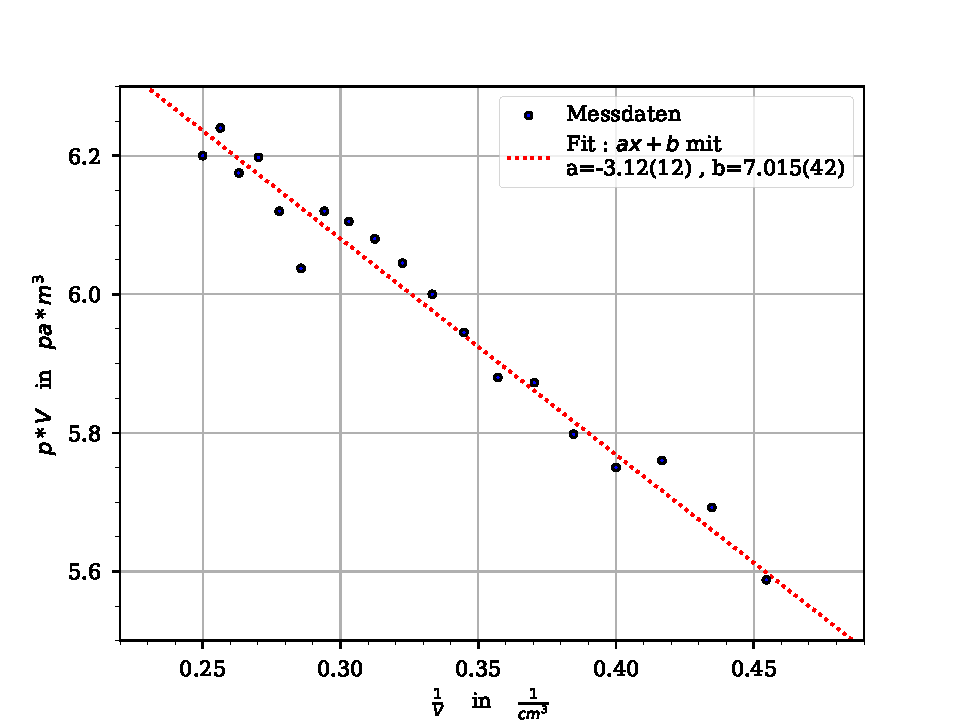
\includegraphics[width=\textwidth]{./Plots/3Plot_n.pdf}

        \caption{Bestimmung der molaren Stoffmenge $n$}
        \label{fig:n}
    \end{figure}
    
    Mithilfe der genauen Messreihe bei $50 \si{\celsius}$ wurde durch einen Fit der
    Funktion \ref{eq:ideal} im Graph \ref{fig:n} die molare Stoffmenge $n = 0,002613(16) \si{\mole}$ bestimmt.
    Diese molare Masse wurde für alle Messreihen benutzt.

    \subsection{Isotherme}
    \begin{figure}
        \centering
        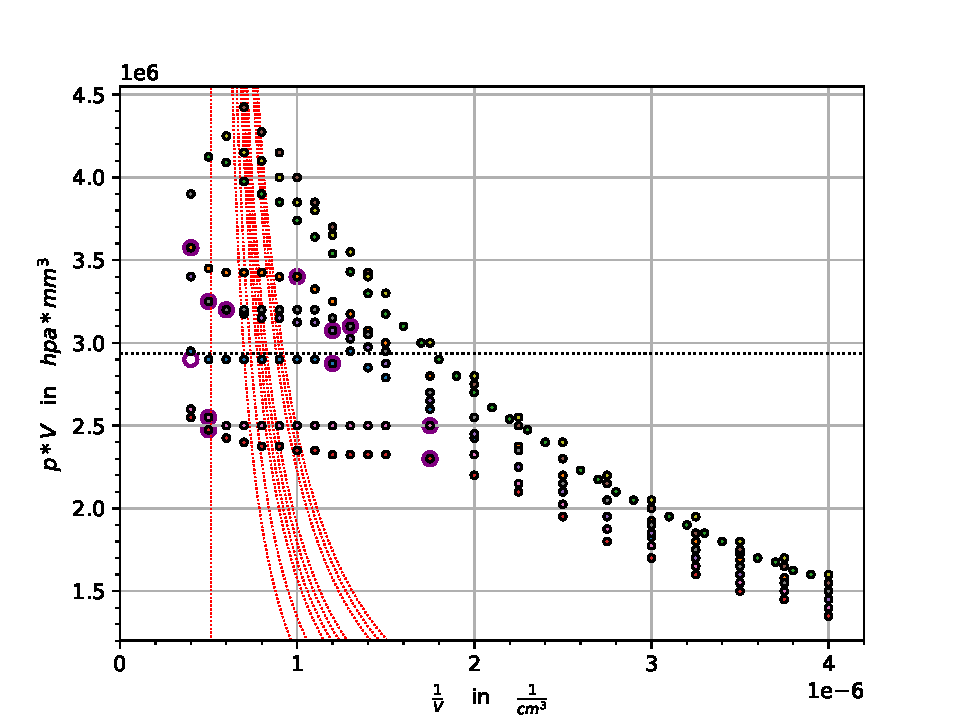
\includegraphics[width=\textwidth]{./Plots/4Plot_of_Hell.pdf}

        \caption{Isotherme bei verschiedenen Temperaturen}
        \label{fig:isotherme}
    \end{figure}
    Die Isothermen sind im Graphen \ref{fig:isotherme} dargestellt, wobei der Druck gegen das Volumen aufgetragen wurde.
    Die Punkte an denen nur noch Gas bzw. Flüssigkeit vorhanden ist, wurden mit einem Kreis markiert. Als
    Unsicherheit wurde die Schrittweite des Thermometers ($\Delta T = 0,1 \si{\celsius} \Rightarrow u_t = 0,028 \si{\celsius}$)
    der Volumenmessung ($\Delta V = 0,05 \si{\milli\liter} \Rightarrow u_v = 0,011 \si{\milli\liter}$) und der Druckmessung
    ($\Delta p = 0,5 \si{\hecto\pascal} \Rightarrow u_p = 0,11 \si{\hecto\pascal}$) verwendet.
    

    \section{Diskussion}
    \begin{table}
        \centering
        \begin{tabular}{c}
            $T_{krit} SF_6 = 45,55 \si{\degree \celsius}$ \cite{SH6} \\
            $p_{krit} SF_6 = 37,53 \si{\bar}$ \cite{SH6} \\
            $\rho_{krit} SF_6 = 735 \si{\kilogram \per \meter \cubed}$ \cite{SH6} \\
            \\
            \begin{tabular}{c c}
                Temperatur in $\si{\degree\celsius}$ & Dampfdruck in $\si{\bar}$ \\ \hline
                20 \si{\celsius} & 2,108 \si{\mega\pascal} \\
                30 \si{\celsius} & 2,66 \si{\mega\pascal} \\
                40 \si{\celsius} & 3,31 \si{\mega\pascal} \\
            \end{tabular}
        \end{tabular}
        \caption{Literaturwerte}
        \label{tab:literaturwerte}
    \end{table}


    \bibliographystyle{plain}
    \bibliography{literature}

\end{document}